\clearpage
\section{Technische Grundlagen Zigbee}\label{sec:TechnischeGrundlagenZigbee}

\subsection{Netzaufbau und Topologie}\label{subsec:NetzaufbauundTopologie}

Zigbee ist nicht gleich Zigbee. Obwohl Zigbee von zentraler Stelle, der Zigbee Alliance, spezifiziert wurde gibt es verschiedene Arten davon. In den Spezifikationen wird zwischen zwei sogenannten Stackprofilen \textit{ZigBee} und \textit{ZigBee PRO} unterschieden.
Während \textit{ZigBee}-Netzwerke eine Baumstruktur haben und der Koordinator dabei einen Single-Point-of-Failure bildet, bieten \textit{ZigBee PRO}-Netzwerke geroutete Mesh Funktionalitäten mit Routing Tabellen und Wegentdeckung. Der Koordinator bildet dabei nicht länger einen Single-Point-of-Failure da sich das Routing dynamisch anpassen kann.
Die Abbildung \ref{fig:NetzwerktopologienZigbee} zeigt die Unterschiede von einem Baumnetzwerk im Stackprofil \textit{ZigBee} links und einem Meshnetzwerk im Stackprofil \textit{ZigBee PRO} rechts.
In der vorliegenden Arbeit wurde das \textit{ZigBee PRO} Stackprofil verwendet womit vollwertige Meshnetzwerke möglich sind.

\begin{figure}[h]
	\centering
	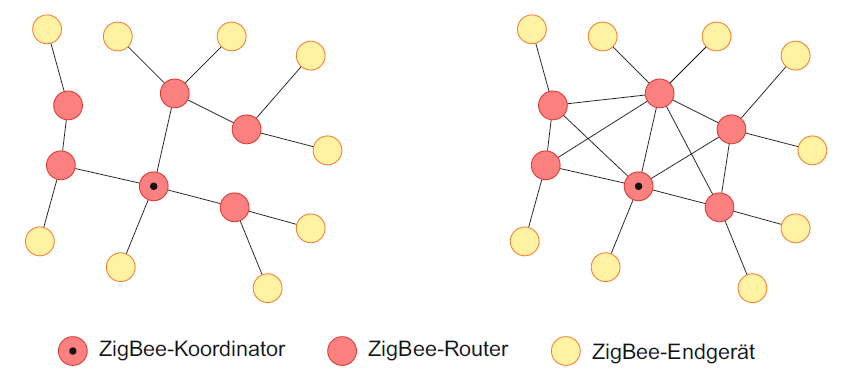
\includegraphics[width=0.8\textwidth]{Zigbee_Netztopologie.png}
	\caption{Zigbee Baum- und Meshnetzwerke \cite[S.~221]{markus_krause_rainer_konrad_zigbee_2014}}	\label{fig:NetzwerktopologienZigbee}
\end{figure}

Wie in der Abbildung \ref{fig:NetzwerktopologienZigbee} bereits angedeutet, kann innerhalb eines Zigbee Meshnetzwerkes zwischen 3 Nodetypen unterschieden werden. Diese besitzen unterschiedliche Aufgaben und Eigenschaften.

\paragraph{Zigbee Koordinator}\label{par:ZigbeeKoordinator}
Als zentrale Einheit übernimmt der \textit{Zigbee Koordinator} Aufgaben wie den Start und die Verwaltung eines PAN (Personal Area Network) inkl. der Definition der wichtigsten Parameter wie der PAN-ID, der Sicherheitsschlüssel sowie die Wahl des IEEE Channels.
In einem Zigbee-Netzwerk gibt es genau ein Gerät das die Rolle des \textit{Zigbee Koordinators} übernimmt. Wenn dieses Gerät das Netzwerk verlässt oder kurzzeitig ausser Betrieb ist, kann das Netzwerk trotzdem weiter bestehen und funktioniert normal weiter.
Jeder \textit{Zigbee-Koordinator} hat gleichzeitig auch die Rolle eines \textit{Zigbee-Router}.

\paragraph{Zigbee Router}\label{par:ZigbeeRouter}
\textit{Zigbee-Router} bilden das eigentliche Meshnetzwerk. Sie übernehmen die Aufgabe des Routings was die Wegentdeckung sowie Weiterleitung von Paketen beinhaltet. Jeder \textit{Zigbee-Router} führt eine Routing-Table welche fortlaufend aktualisiert wird.

\paragraph{Zigbee End-Device}\label{par:ZigbeeEndDevice}
Die einfachste Rolle ist jene des \textit{Zigbee End-Devices}. Sie stehen in einer Parent-Child Beziehung mit einem \textit{Zigbee-Router}.
Diese Kommunikation findet entweder periodisch oder ausgelöst durch einen Userinput statt.
Ankommende Pakete werden jeweils vom Parent-Node gespeichert bis das  \textit{Zigbee End-Devices} diese abruft.
\textit{Zigbee End-Devices} besitzen ausserdem keine Routing Funktionen und gelten deshalb als sehr energiesparend.
Ausgeführt als Sleepy-End-Device können CPU und RAM des entsprechenden Nodes ganz oder teilweise heruntergefahren werden und durch periodische Interrupts geweckt werden.
Dadurch können sehr lange Batteriestandzeiten erreicht werden. \cite{markus_krause_rainer_konrad_zigbee_2014}


\subsection{Zigbee Protokoll Stack}\label{subsec:ZigbeeProtokollStack}

Die Architektur des Zigbee Stacks besteht aus vier Layern, dem Physical layer (PHY), dem MAC layer, dem Network layer (NWK) und dem Application layer (APL).
Abbildung \ref{fig:ArchitekturdesZigbeeProtokollStacks} zeigt den Aufbau des Protokoll Stacks im Detail.
Jede der Schichten ist mit bestimmten Aufgaben betraut und stellt der darüber liegenden Schicht Daten und Dienste bereit.
Nachfolgend wird auf die vier Schichten des Zigbee Stacks eingegangen und deren Funktion und Funktionsweise kurz erläutert.

\begin{figure}[h]
	\centering
	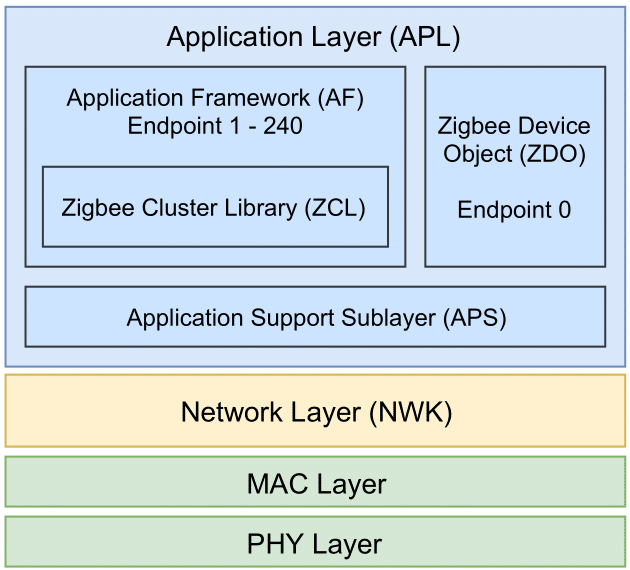
\includegraphics[width=0.7\textwidth]{Zigbee_Architektur.png}
	\caption{Architektur des Zigbee Protokoll Stacks}
	\label{fig:ArchitekturdesZigbeeProtokollStacks}
\end{figure}

\subsubsection{MAC und PHY Layer}\label{subsubsec:MACundPHYLayer}
Der MAC und Physical Layer (PHY) werden im Zigbee Protokoll Stack gebildet durch den IEEE 802.15.4 Standard für \textit{Wireless Personal Area Networks} (WPAN).
Während beispielsweise Wifi oder Bluetooth, welche auf dem selben 2.4 GHz ISM-Funkfrequenzband betrieben werden können, für hohe Datenübertragungsraten konzipiert wurden, ist dieser Standard für kleinere Datenmengen optimiert.
Durch die Vermeidung von unnötigen Steuerinformationen, kann der IEEE 802.15.4 Standard auf einfachster Hardware realisiert und mit kleinstem Energieaufwand betrieben werden.
Ideal also für sogenannte \textit{Wireless Sensor Networks} (WSN) wie beispielsweise Zigbee. \cite{markus_krause_rainer_konrad_ieee_2014}


\subsubsection{Network Layer}\label{subsubsec:Network Layer}
Der Network Layer ist im Zigbee Stack verantwortlich für den Aufbau sowie das Management der Netzwerkfunktionen und das Routing innerhalb dieses Netzwerkes.

\paragraph{Netzaufbau und Adressierung}\label{par:ZigbeeNetzaufbauundAdressierung}
Wie unter \ref{par:ZigbeeKoordinator} bereits erwähnt ist der Koordinator verantwortlich für den Aufbau des Zigbee Netzwerks und der Wahl von entsprechend geeigneten Parametern wie beispielsweise einer 16-Bit PAN-ID oder eines möglichst störungsfreien Funkkanals.
Beim Beitritt eines neuen Funkmoduls wird diesem vom Koordinator eine im Netzwerk einmalige 16-Bit \textit{Short-Address} zugewiesen.
Anhand dieser kann das Funkmodul nun im Netzwerk adressiert werden und es selbst kann damit Routing Funktionen war nehmen.
Die im MAC Layer definierte 64-Bit MAC Adresse kann ebenfalls vollwertig für die Adressierung verwendet werden wobei diese schliesslich in die \textit{Short-Address} übersetzt wird.


\paragraph{Routing}\label{par:Zigbee Routing}
Das Routing geschieht innerhalb von Zigbee Mesh Netzwerken mit dem \textit{ZigBee PRO}-Stackprofil mittels Routingtabellen die jeder Router erstellt und nach führt wenn es Änderungen gibt. In dieser ist die \textit{Short-Address} des Ziels sowie jene des nächsten Hops hinterlegt.
Enthält die Routingtabelle veraltete Einträge oder sind für das entsprechende Ziel noch gar keine Informationen vorhanden, muss ein \textit{Route Discovery} durchgeführt werden.
Hierbei handelt es sich um eine Broadcast Nachricht welche an alle Router gesendet wird. Diese empfangen die Nachricht und leiten sie wiederum als Broadcast an alle Router in Reichweite weiter. Dabei werden die Wegkosten jeweils addiert um diese sobald die Nachricht beim Zielnode angekommen ist, dem Absender mitzuteilen.
So wird jener Weg mit den geringsten totalen Wegkosten ermittelt und kann schliesslich in der Routingtabelle abgelegt werden.


\subsubsection{Application Layer (APL)}\label{subsubsec:ZigbeeApplicationLayer}
Der Zigbee Application Layer kann in drei Teile unterteilt werden, den Application Support Sublayer, das Zigbee Device Object und das Application Framework mit der Zigbee Cluster Library als eigentliche Anwendung.

\paragraph{Application Support Sublayer (APS)}\label{par:ZigbeeApplicationSupportSublayer}
Wie der Name andeutet ist der APS Layer für die Anwendungsunterstützung zuständig und ist als Zwischenschicht im Application Layer eingebettet.
Zu den Aufgaben des APS Layers gehören das Binding, das Gruppenmanagement, die Datenübertragung inkl. Fragmentierung sowie das Erstellen und Versenden von APS-Frames.
Ausserdem bietet der APS Layer eine Möglichkeit der Empfangsbestätigung auf Applikationsebene. Anders als die Empfangsbestätigung auf MAC Ebene ist diese nicht nur auf Funkmodule in unmittelbarer Reichweite beschränkt.

\begin{figure}[h]
	\centering
	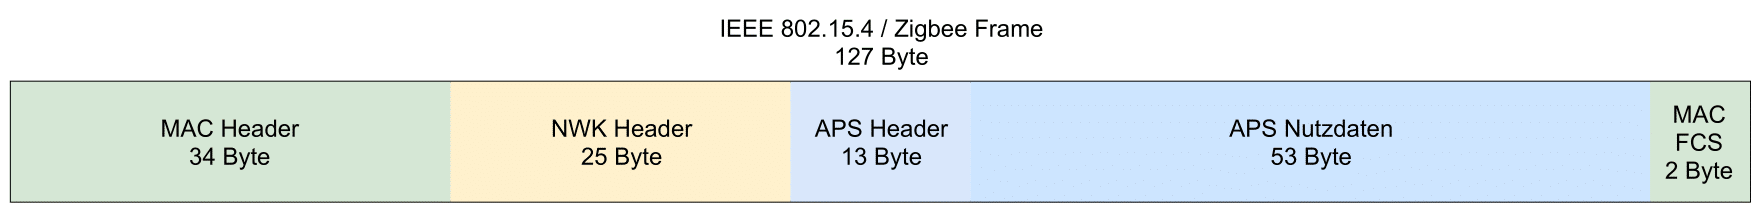
\includegraphics[width=\textwidth]{Zigbee_Frame_Structure.png}
	\caption{Zigbee Frame Struktur bei aktivierten Sicherheitsfunktionen \cite[S.~286]{markus_krause_rainer_konrad_zigbee_2014}}
	\label{fig:ZigbeeFrameStruktur}
\end{figure}

Die Fragmentierung von APS Nutzdaten basiert darauf, dass die Grösse von Frames durch den PHY Layer auf 127 Byte beschränkt ist.
Abzüglich sämtlicher Header auf MAC, NWK sowie APS Ebene und sonstigem Protokoll Overhead beispielsweise hinsichtlich Sicherheit, reduziert sich die nutzbare APS-Payload Grösse auf 53 Byte (siehe Abbildung \ref{fig:ZigbeeFrameStruktur}).
Sollen nun grössere Daten übertragen werden führt der APS Layer eine Fragmentierung durch \cite[S.~279 - 299]{markus_krause_rainer_konrad_zigbee_2014}.


\paragraph{Application Framework (AF) mit Zigbee Cluster Library (ZCL)}\label{par:ZigbeeAFZCL}
Das Application Framework bildet den Bereich des APL in dem die eigentlichen Anwendung abläuft. Für die Adressierung stehen dem Anwender dabei 240 sogenannte Endpoints zur Verfügung. Endpoints können mit dem Prinzip von Ports im TCP/IP Modell verglichen werden.
Sie dienen dazu unterschiedliche Anwendungen auf dem selben Node zu adressieren.
Innerhalb des AF können Anwendungen nun prinzipiell frei umgesetzt werden.
Um den Herstellern jedoch eine herstellerunabhängige Applikationsentwicklung zu ermöglichen, wurde durch die Zigbee Alliance die \textit{Zigbee Cluster Library (ZCL)} spezifiziert.
Anwendungen wie beispielsweise ein Lichtschalter, werden durch sogenannte Cluster detailliert beschrieben.
Dabei handelt es sich um eine Sammlung von Kommandos und Attributen für den jeweiligen Anwendungszweck.

\paragraph{Zigbee Device Object (ZDO)}\label{par:ZigbeeDeviceObject}
Das Zigbee Device Object ist ein eigenständiges Anwendungsobjekt welches immer mit dem Endpoint 0 addressiert wird.
Es setzt die Funktionalitäten gemäss Definition der Zigbee Rollen (Koordinator, Router, Enddevice) um und benutzt dafür Funktionen der NWK sowie APS Schicht.
Beispielsweise ist es zuständig für das Netzwerkmanagement, Knotenmanagement und auch für die Implementation von Sicherheitsfunktionen.

\subsubsection{Sicherheit}\label{subsucsec:ZigbeeSicherheit}
\todo[inline]{Sicherheitsmechanismus beschreiben.}


\subsection{Zigbee Software Development Kit}\label{subsec:ZigbeeSoftwareDevelopmentKit}
\todo[inline]{Eingesetzte SDK und deren Aufbau beschreiben. Allenfalls die wichtigsten API Funktionen genauer erläutern.}

Für die Umsetzung von Zigbee Applikationen auf dem nRF52840 SoC \ref{subsec:SystemonChip} stellt Nordic Semiconductor ein eigenes Software Development Kit (SDK) zur Verfügung, die \textit{nRF5 SDK for Thread and Zigbee} \cite{nordic_semi_nrf_sdk_for_thread_and_zigbee_2020}.
Da Thread und Zigbee den selben IEEE 802.15.4 MAC Layer benutzen, teilen sich die beiden Protokollstacks eine gemeinsame SDK.
Innerhalb der SDK nutzen die beiden jedoch unterschiedliche Ressourcen.

\begin{figure}[h]
	\centering
	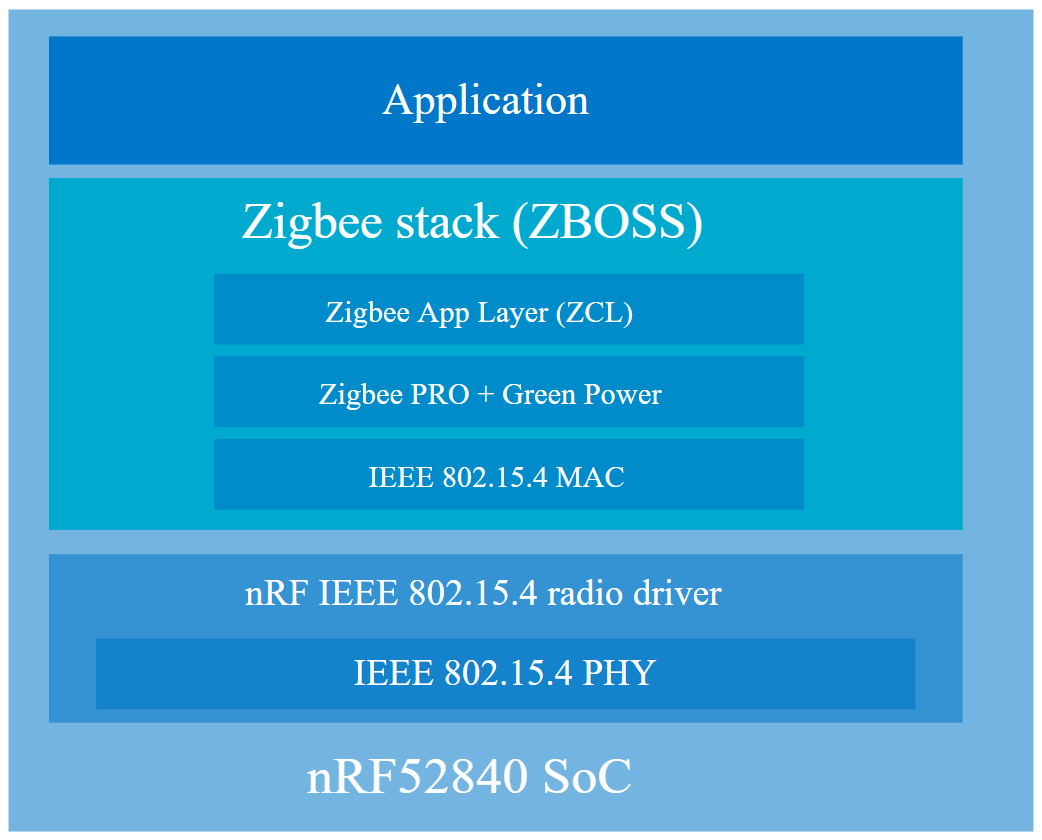
\includegraphics[width=0.6\textwidth]{Zigbee_SDK_Plattform_Design.png}
	\caption{nRF5 SDK for Thread and Zigbee Plattform Design Referenz für Zigbee Applikationen \cite{nordic_semi_nrf_sdk_for_thread_and_zigbee_2020}}
	\label{fig:ZigbeePlattformDesign}
\end{figure}

Für Zigbee Applikationen kommt ein Plattform Design gemäss Abbildung \ref{fig:ZigbeePlattformDesign} zum Einsatz. 
Als eigentlicher Zigbee Stack kommt dabei der \textit{ZBOSS} Zigbee Stack in der Version 3.3 von DSR\footnote{ZBOSS stack v3.3.0: \url{https://dsr-iot.com/}} zum Einsatz.
Es handelt sich dabei um einen weit verbreiteten \textit{Zigbee PRO} Stack welcher die neuste Version der Zigbee Core Specification rev22 umsetzt.
\textit{ZBOSS} verwendet dabei ein kooperatives Multitasking Prinzip mit einem Scheduler welche die aktiven Tasks verwaltet.

Unter dem \textit{ZBOSS} Stack verwendet die SDK den \textit{nRF IEEE 802.15.4 radio driver} für die Ansteuerung der Funkschnittstelle.
Oberhalb des \textit{ZBOSS} Stacks befindet sich die Applikationsebene in welcher unter anderem ZCL Funktionen auch aus \textit{ZBOSS} verwendet werden können.


 

 